\section{Comparaisons de performance et de qualité}

\begin{frame}
    \tableofcontents[currentsection]
\end{frame}

\begin{frame}
\frametitle{Comparaison de l'efficacité}
\framesubtitle{A basse / moyenne précision}
\begin{figure}
    \centering
    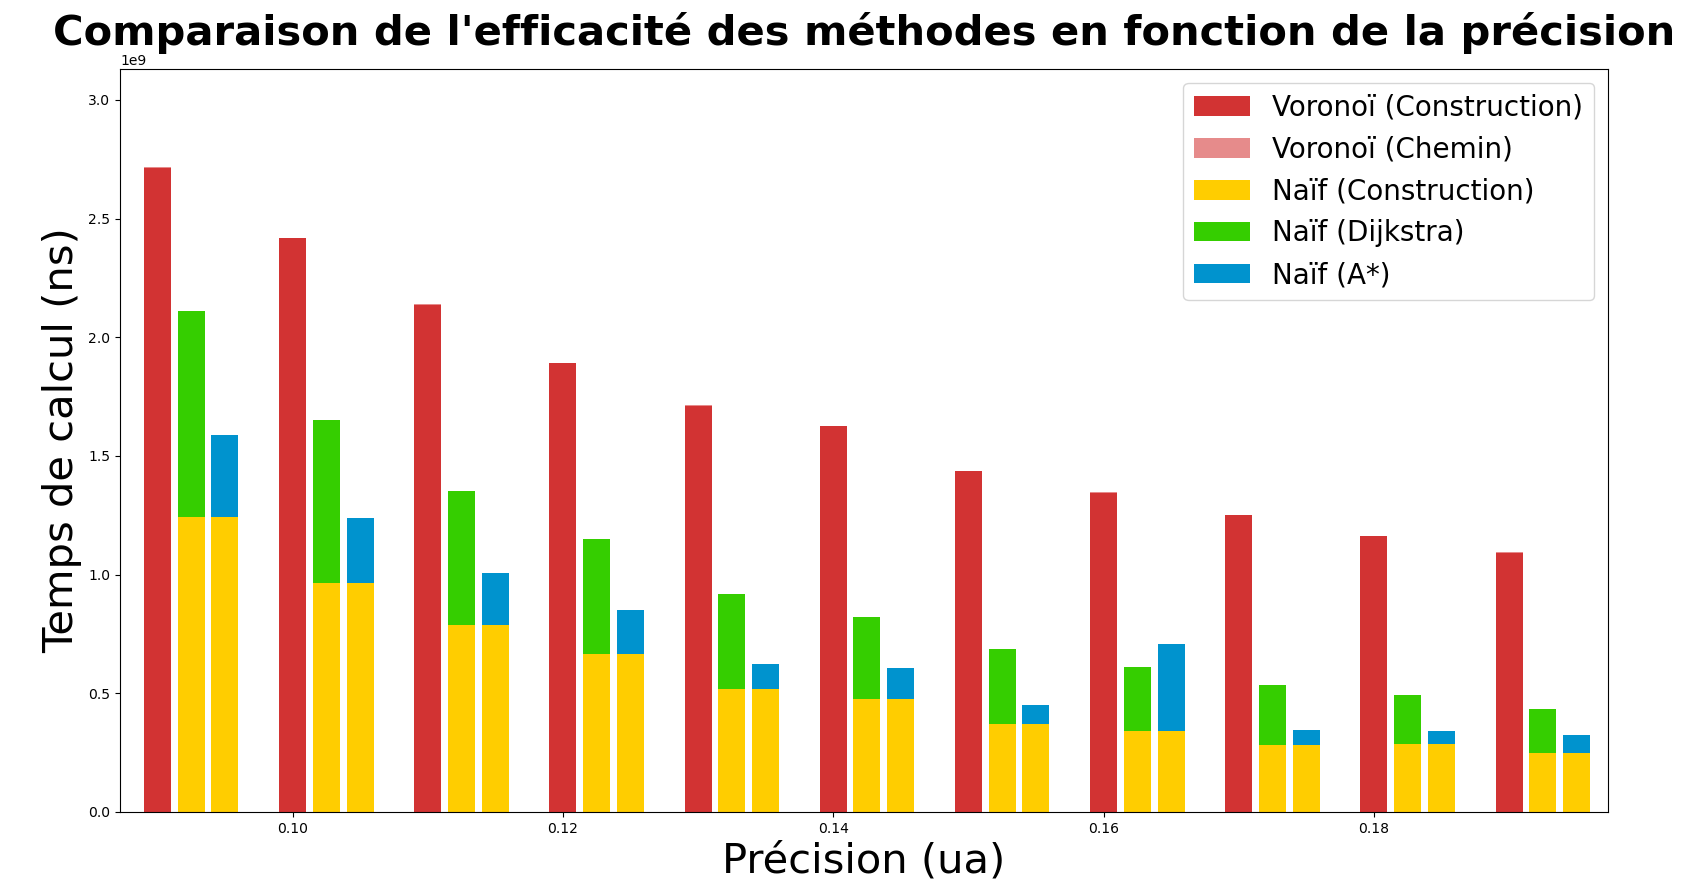
\includegraphics[width=1\linewidth]{assets/BassePrecision.png}
    % \caption{Caption}
\end{figure}
\end{frame}


\begin{frame}
\frametitle{Comparaison de l'efficacité}
\framesubtitle{Mais quand on regarde à haute précision...}
\begin{figure}
    \centering
    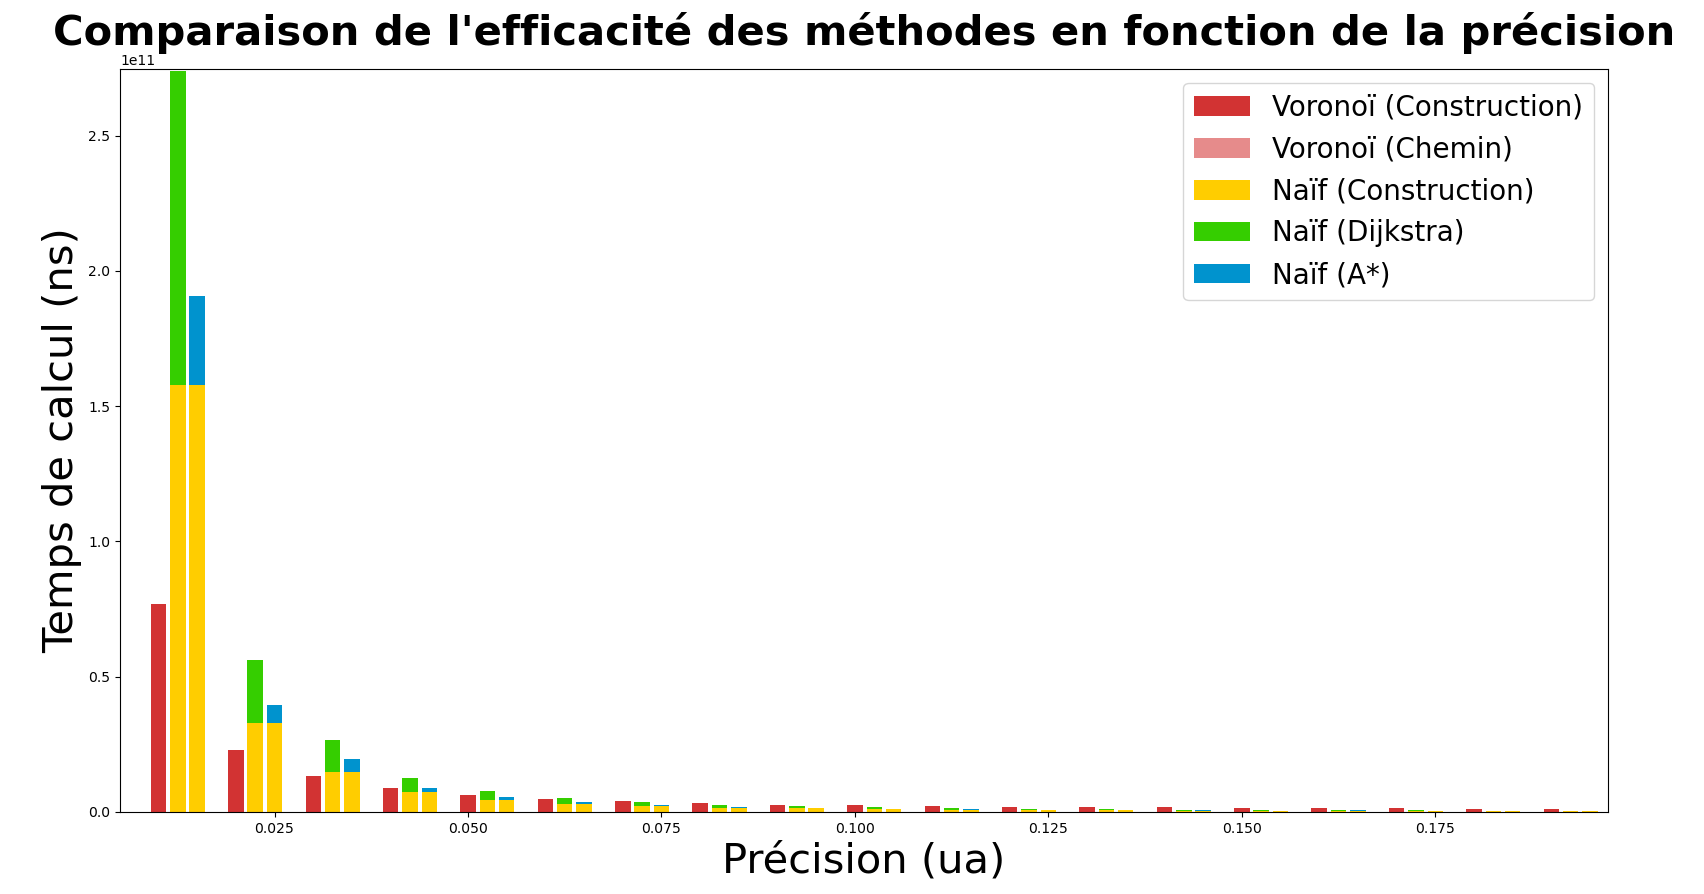
\includegraphics[width=1\linewidth]{assets/ToutesPrecision.png}
    % \caption{Caption}
\end{figure}
\end{frame}

\begin{frame}
\frametitle{Comparaison de la qualité}
\begin{table}
\begin{tabular}{|c||c|c|}
    \hline
     - & Naïf & Voronoï \\
    \hline\hline
    \begin{sideways}
    Basse résolution~
    \end{sideways}
    &
    \begin{figure}
        \centering
        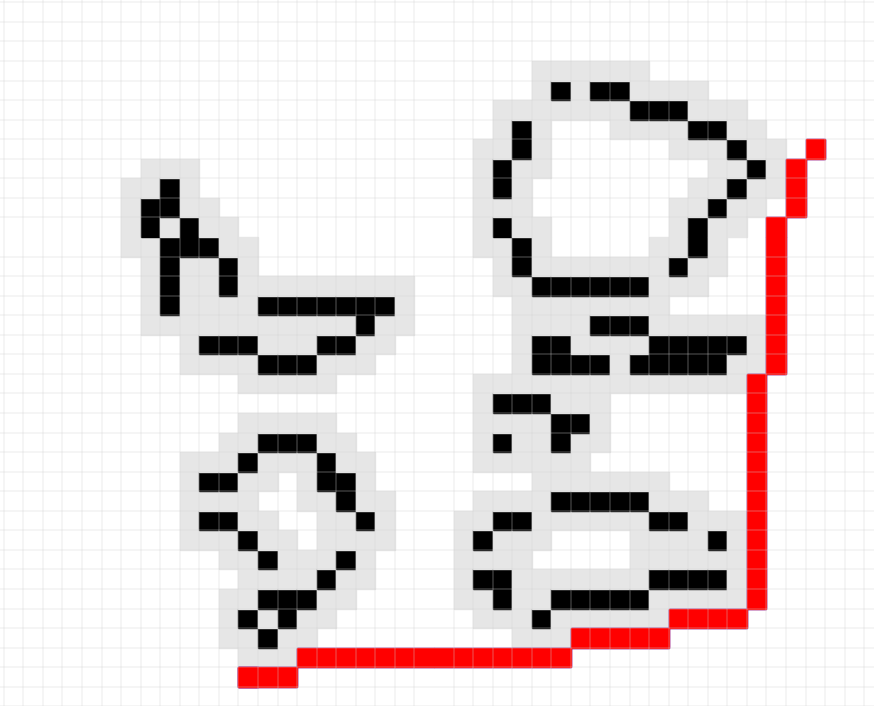
\includegraphics[width=0.3\linewidth]{assets/NaLow.png}
    \end{figure}
    &
    \begin{figure}
        \centering
        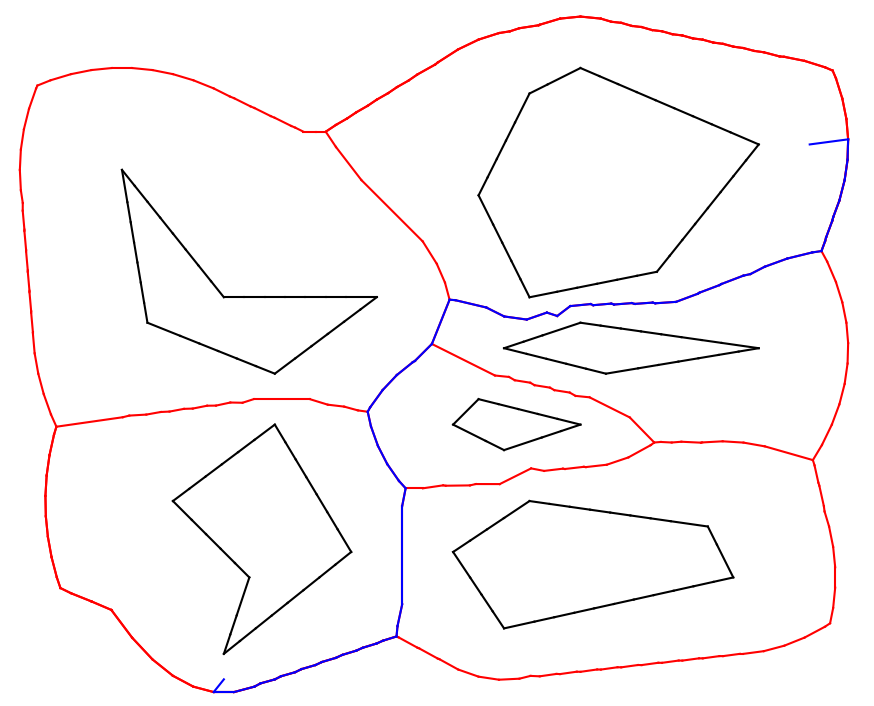
\includegraphics[width=0.3\linewidth]{assets/VorLow.png}
    \end{figure} \\
    \hline
    \begin{sideways}
    Haute résolution~
    \end{sideways}
    &
    \begin{figure}
        \centering
        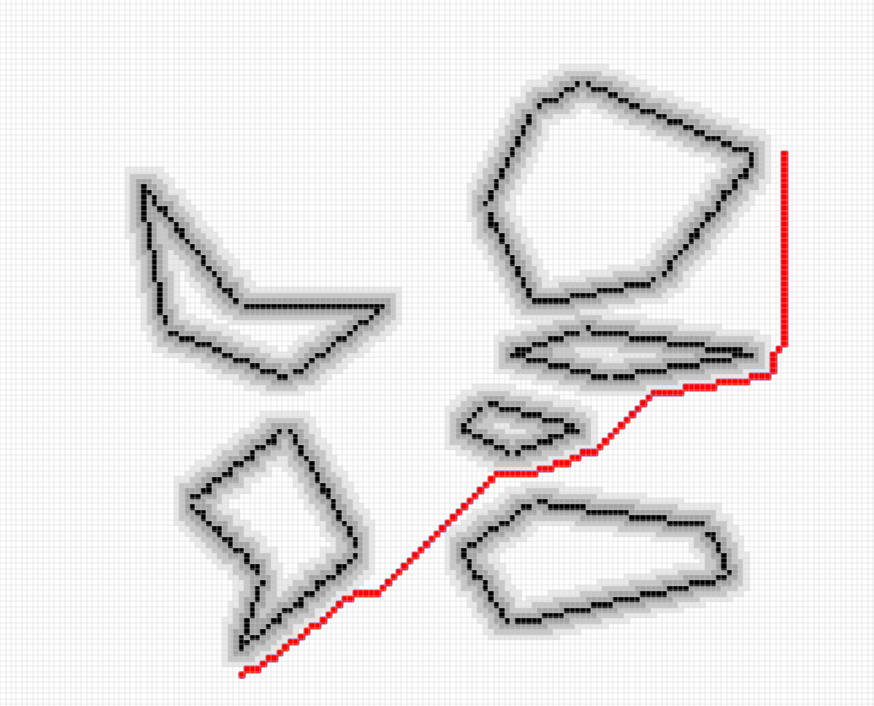
\includegraphics[width=0.3\linewidth]{assets/NaHigh.png}
    \end{figure}
    &
    \begin{figure}
        \centering
        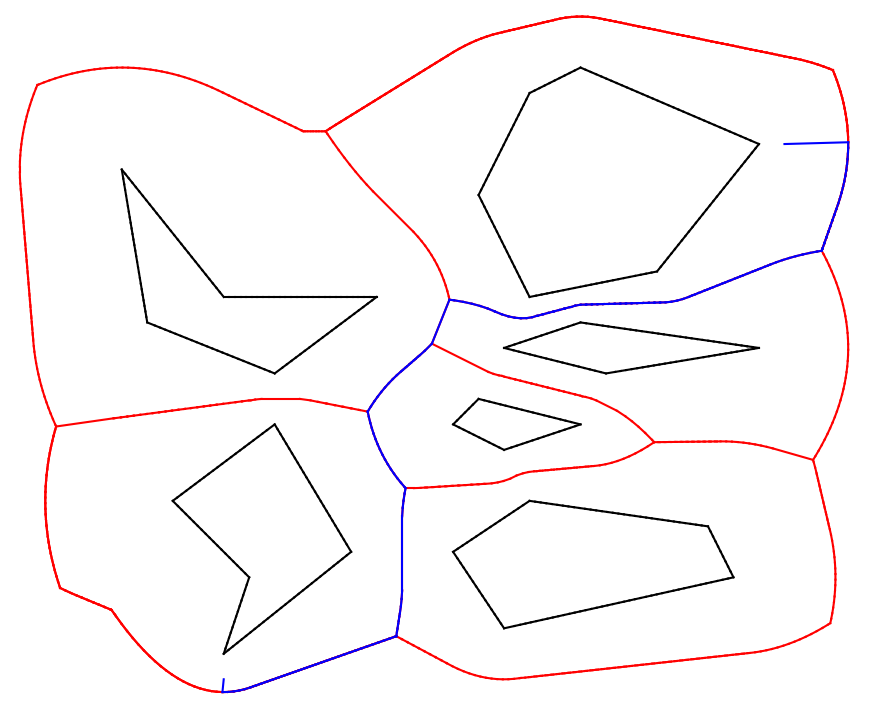
\includegraphics[width=0.3\linewidth]{assets/VorHigh.png}
    \end{figure} \\
    \hline
\end{tabular}
\end{table}
\end{frame}